\section{Baseline with Middleware (90 pts)}

% In this set of experiments, you will have to use three load generator VMs and 1 memcached server, measuring how the throughput of the system changes when increasing the number of clients. Scaling virtual clients inside memtier has to be done as explained in the previous sections. Plot both throughput and response time as measured on the middleware.

In this section, we study the performance characteristics of the system with one or two middlewares added between memtier and memcached.


\subsection{One Middleware}

In this subsection, we study the performance characteristics of one middleware, with three load generating machines and one memcached server. We compare it with baselines in Section 2.1, which has a similar setup except that it has no middlewares involved. Below is the experiment setup.

\begin{center}
	\scriptsize{
		\begin{tabular}{|l|c|}
			\hline Number of servers                & 1                        \\ 
			\hline Number of client machines        & 3                        \\ 
			\hline Instances of memtier per machine & 1                        \\ 
			\hline Threads per memtier instance     & 2                        \\
			\hline Virtual clients per thread       & [1,2,3,4,6,8,16,32]; For write-only [24] in addition \\
			\hline Workload                         & Write-only and Read-only \\
			\hline Multi-Get behavior               & N/A                      \\
			\hline Multi-Get size                   & N/A                      \\
			\hline Number of middlewares            & 1                        \\
			\hline Worker threads per middleware    & [8,16,32,64]                  \\
			\hline Repetitions                      & 3 $\times$ 80 seconds each                \\ 
			\hline 
		\end{tabular}
	} 
\end{center}


\begin{figure}[!h]
\parbox{.5\linewidth}{
\centering
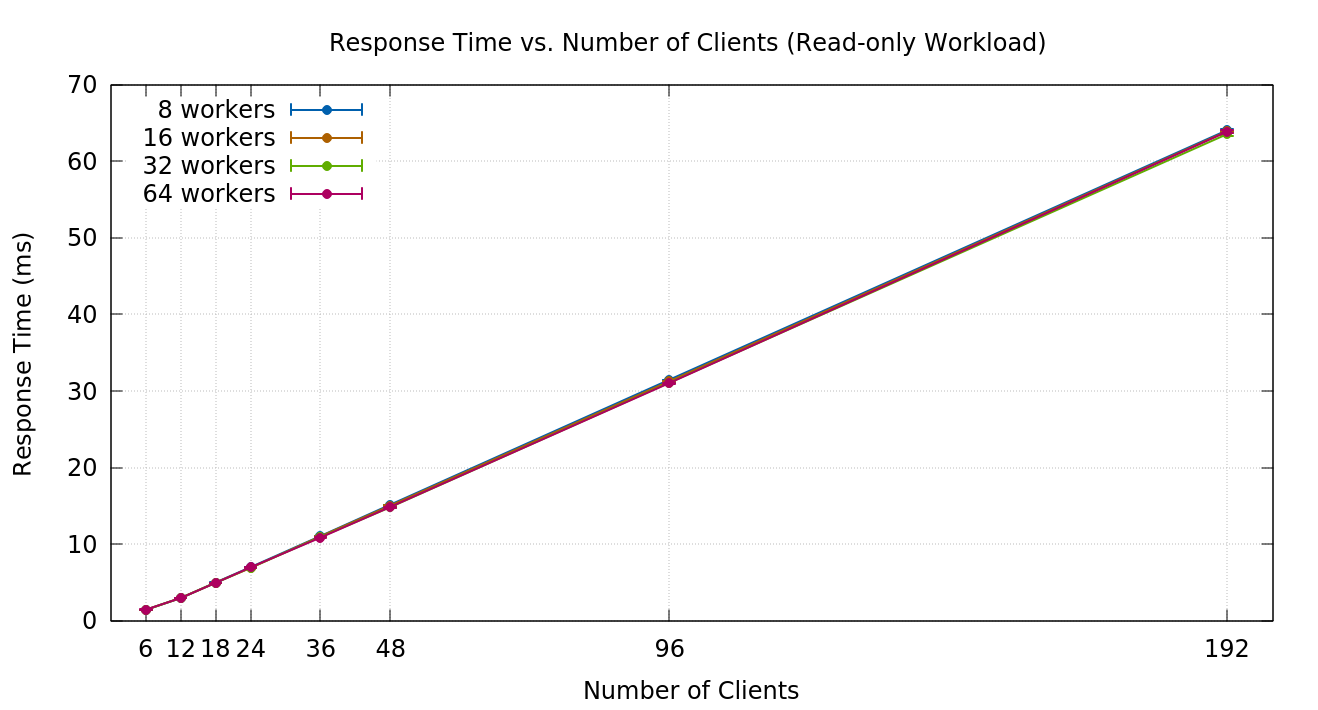
\includegraphics[width=0.5\textwidth]{img/3_1_responsetime_readonly_mw.png}
}
\parbox{.5\linewidth}{
\centering
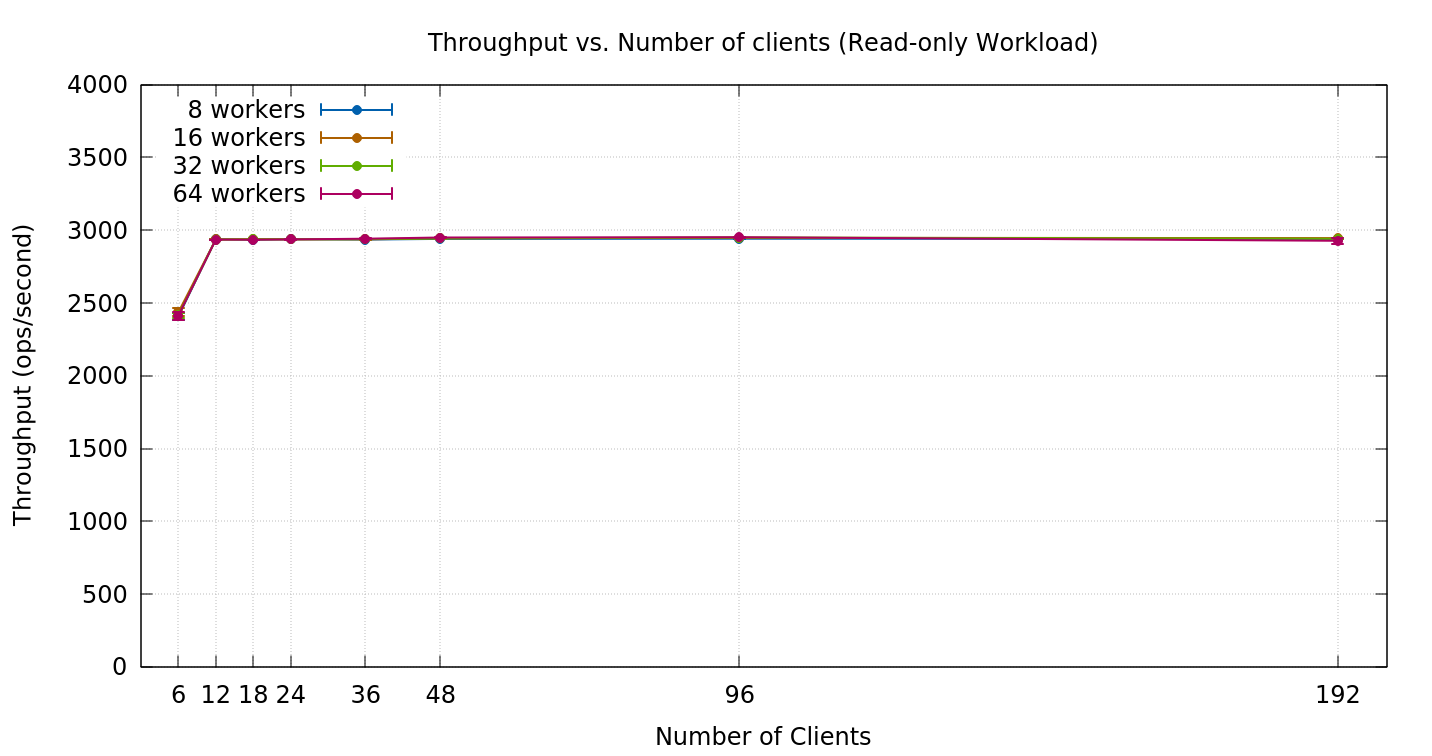
\includegraphics[width=0.5\textwidth]{img/3_1_throughput_readonly_mw.png}
}
\captionsetup{justification=centering}
\caption{\label{fig:3.1readonly_mw}One Middleware Read-only Response Time and Throughput Measured on Middleware \\(Error bars are too small to be distinguished)}
% \end{figure}

% \begin{figure}[!h]
\parbox{.5\linewidth}{
\centering
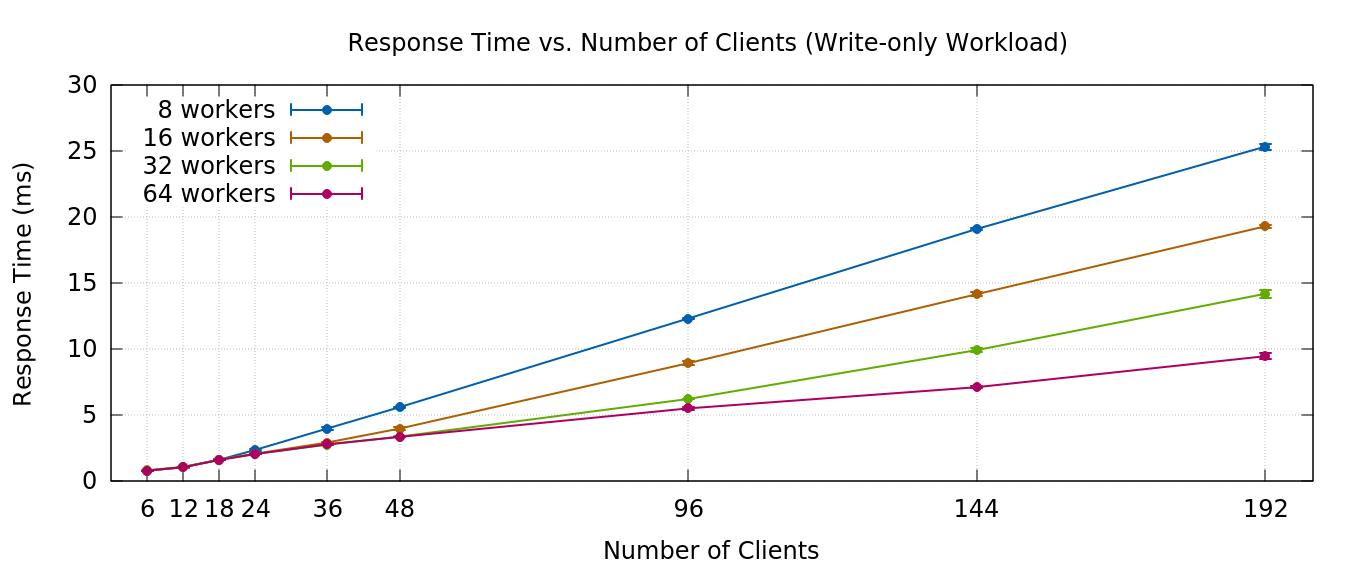
\includegraphics[width=0.5\textwidth]{img/3_1_responsetime_writeonly_mw.png}
}
\parbox{.5\linewidth}{
\centering
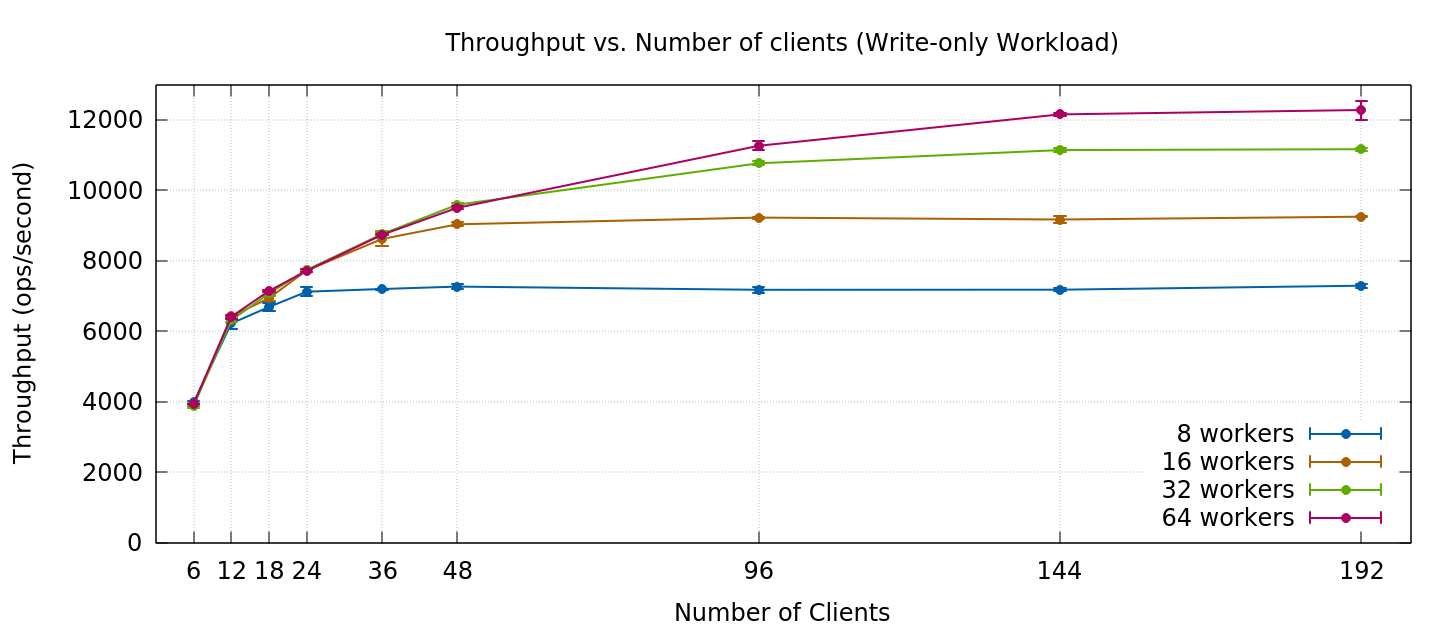
\includegraphics[width=0.5\textwidth]{img/3_1_throughput_writeonly_mw.png}
}
\captionsetup{justification=centering}
\caption{\label{fig:3.1writeonly_mw}One Middleware Write-only Response Time and Throughput Measured on Middleware \\(Error bars are too small to be distinguished)}
% \end{figure}

% % \begin{figure}[!h]
% \parbox{.5\linewidth}{
% \centering
% 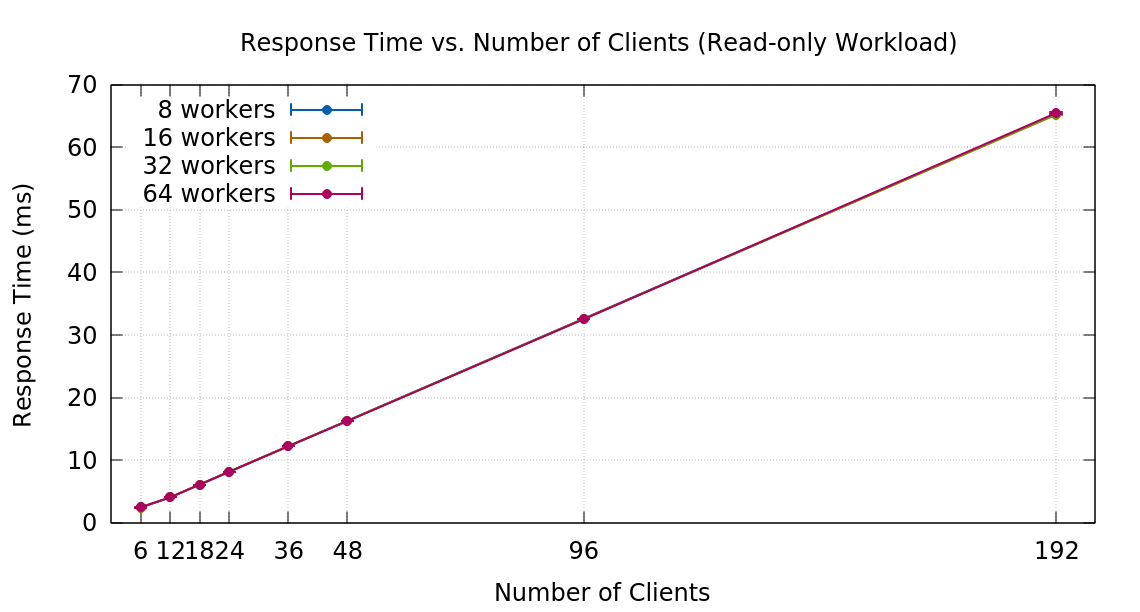
\includegraphics[width=0.5\textwidth]{img/3_1_responsetime_readonly_client.png}
% }
% \parbox{.5\linewidth}{
% \centering
% 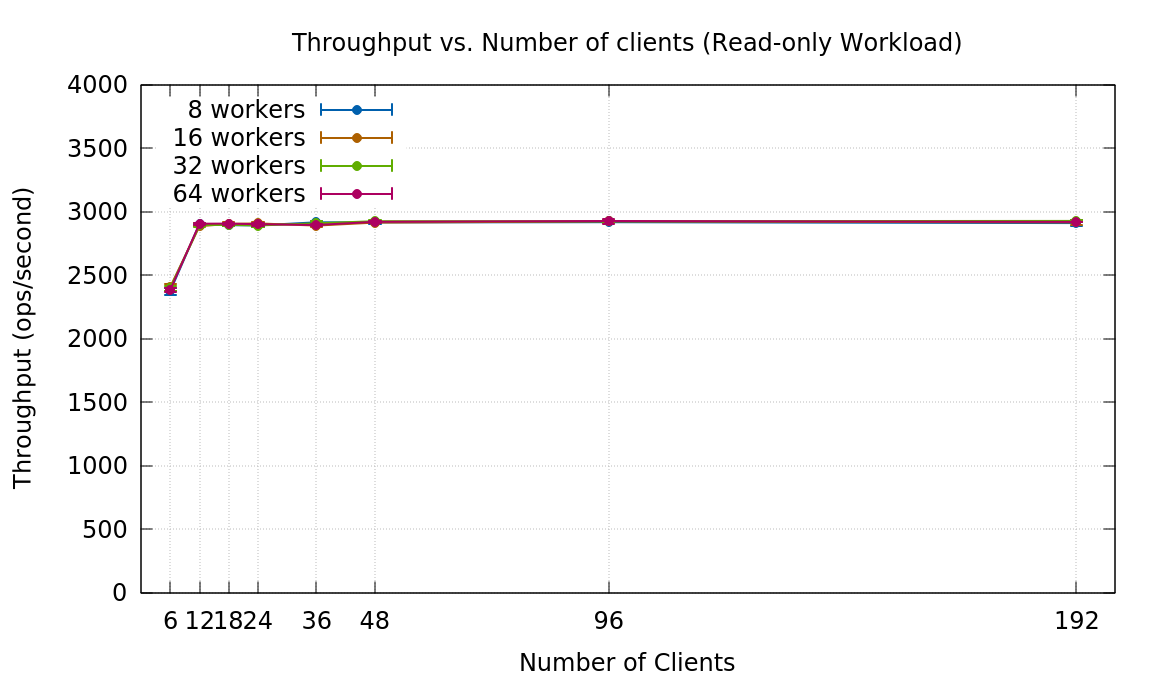
\includegraphics[width=0.5\textwidth]{img/3_1_throughput_readonly_client.png}
% }
% \captionsetup{justification=centering}
% \caption{\label{fig:3.1readonly_client}One Middleware Read-only Performance Measured on Memtier \\(Error bars are too small to be distinguished)}
% % \end{figure}

% % \begin{figure}[!h]
% \parbox{.5\linewidth}{
% \centering
% 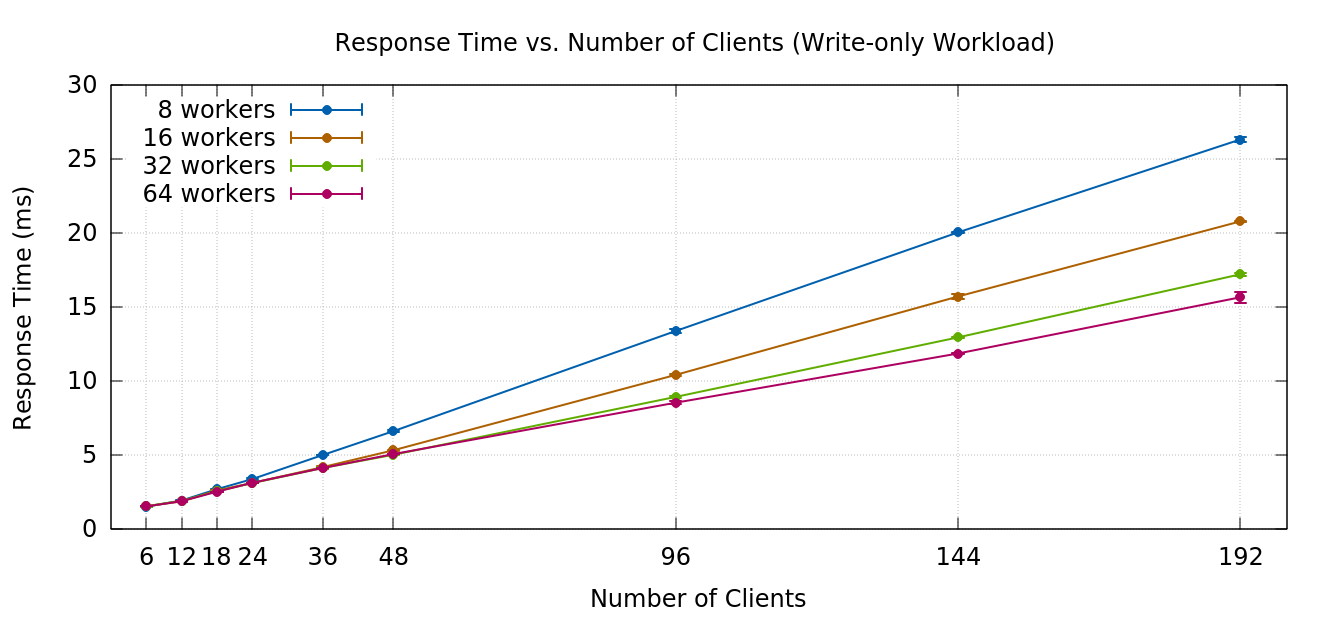
\includegraphics[width=0.5\textwidth]{img/3_1_responsetime_writeonly_client.png}
% }
% \parbox{.5\linewidth}{
% \centering
% 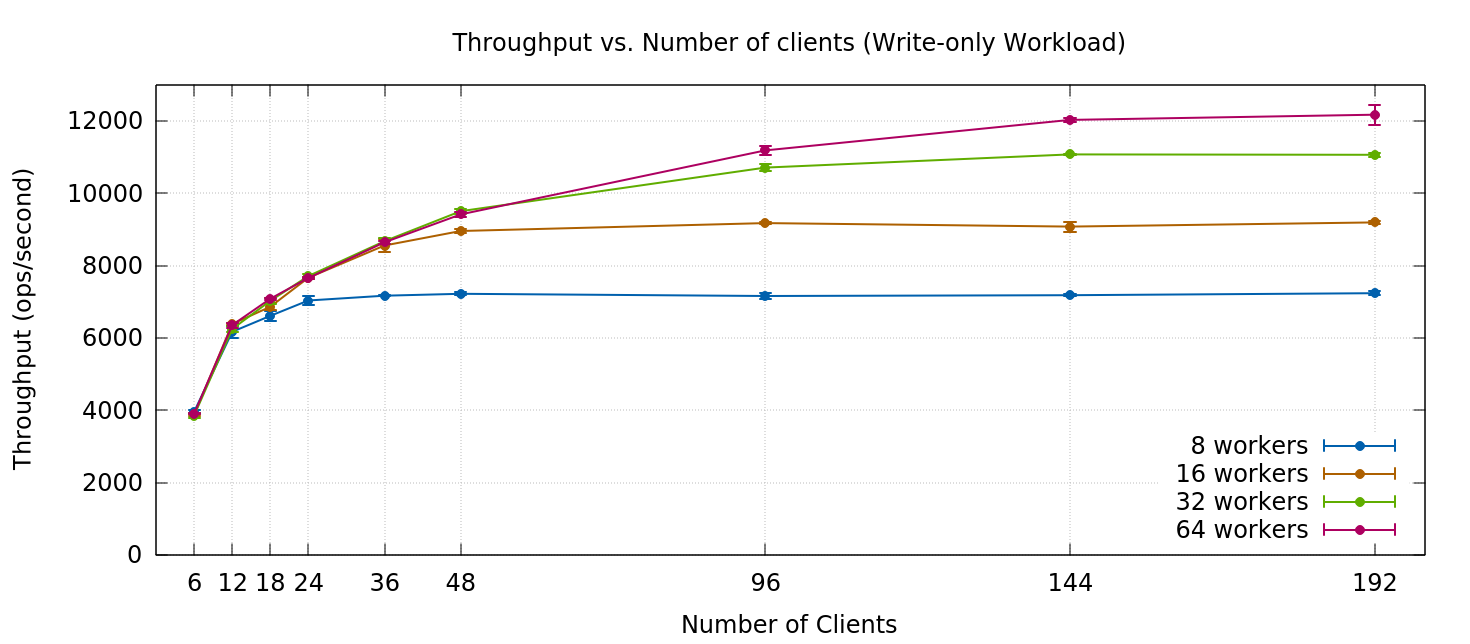
\includegraphics[width=0.5\textwidth]{img/3_1_throughput_writeonly_client.png}
% }
% \captionsetup{justification=centering}
% \caption{\label{fig:3.1writeonly_client}One Middleware Write-only Performance Measured on Memtier \\(Error bars are too small to be distinguished)}

\end{figure}

Figure~\ref{fig:3.1readonly_mw} is the response time and throughput measured by the middleware with regard to the number of clients, for read-only workload. Figure~\ref{fig:3.1writeonly_mw} is for write-only workload. By calculating the theoretical throughput from the number of clients and the memtier-measured response time, and comparing it with the memtier-measured throughput, we confirm that \textbf{the interactive law holds} for memtier clients. 

However, for the middleware, the interactive law does not automatically hold by simply using the number of memtier virtual clients and the middleware-measured response time, because the middleware-measured response time is not the of the whole system, but of the sub-system where the middleware works as clients and memcached works as server. There exist two ways to fix this: either to adapt the number of clients, which is smaller than the number of memtier clients, or to add a think time, because between one request is completed and the next request is ready, there is a time gap, which could be contributed by various factors, including network latency and the waiting time when the network thread is too busy. 

For the first approach, the real number of clients (requests) in the sub-system should be the number of waiting-in-queue requests ($N_q$) plus the number of requests being served ($N_s$). $N_s$ is equal to the number of ``active" threads, which can be less than the number of worker threads, possibly due to middleware saturation or insufficient number of requests. If we take the active worker threads and the server as another sub-system, by definition the number of active workers is the product of throughput and service time measured at the middleware. Therefore, using $N_q + N_s$ as the number of clients, the interactive law is verified to hold for the middleware.

For the second approach, we take the response time difference between memtier and middleware measurements, which is exactly the network round trip time plus any waiting time before a request is read into the network thread, as the think time $Z$, and the interactive law is again verified to hold for the middleware.


\subsubsection{Explanation}

The results are consistent with the baseline measurements in Section 2.1, in that the maximum throughputs are always lower than the case without middleware, and response times are a bit higher due to the added network and processing latency.

For read-only workload, the saturation point, which is 12 clients, comes later than the 6 clients in Section 2.1, because the network latency is roughly doubled as we now have an additional node in the middle, making it not enough to be hidden with just 6 clients. But as soon as we have enough parallelism as 12 clients, the system is again saturated, with the response time growing linearly while throughput staying unchanged, due to the bottleneck at the memcached server's sending bandwidth. The middleware never becomes the bottleneck, as we can see from Figure~\ref{fig:3.1readonly_mw}, even 8 workers are able to achieve the maximum throughput of 2937.96 ops/sec.

\begin{figure}[!h]
\centering
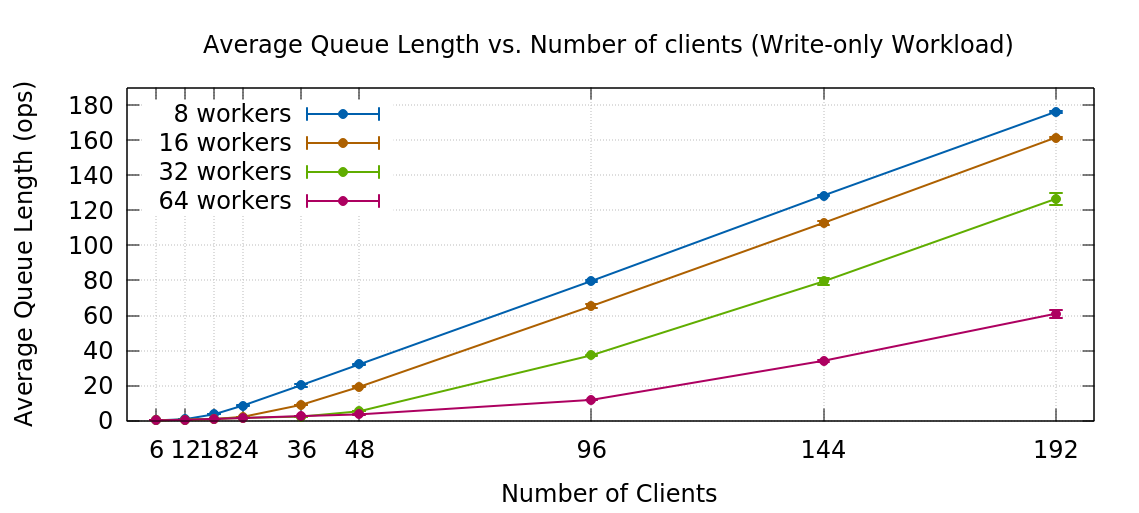
\includegraphics[width=0.75\textwidth]{img/3_1_queuelen_writeonly.png}
\captionsetup{justification=centering}
\caption{\label{fig:3.1writeonly_queue}Average Queue Length for One Middleware Write-only Workload \\(Error bars are too small to be distinguished)}
% \end{figure}

% \begin{figure}[!h]
\centering
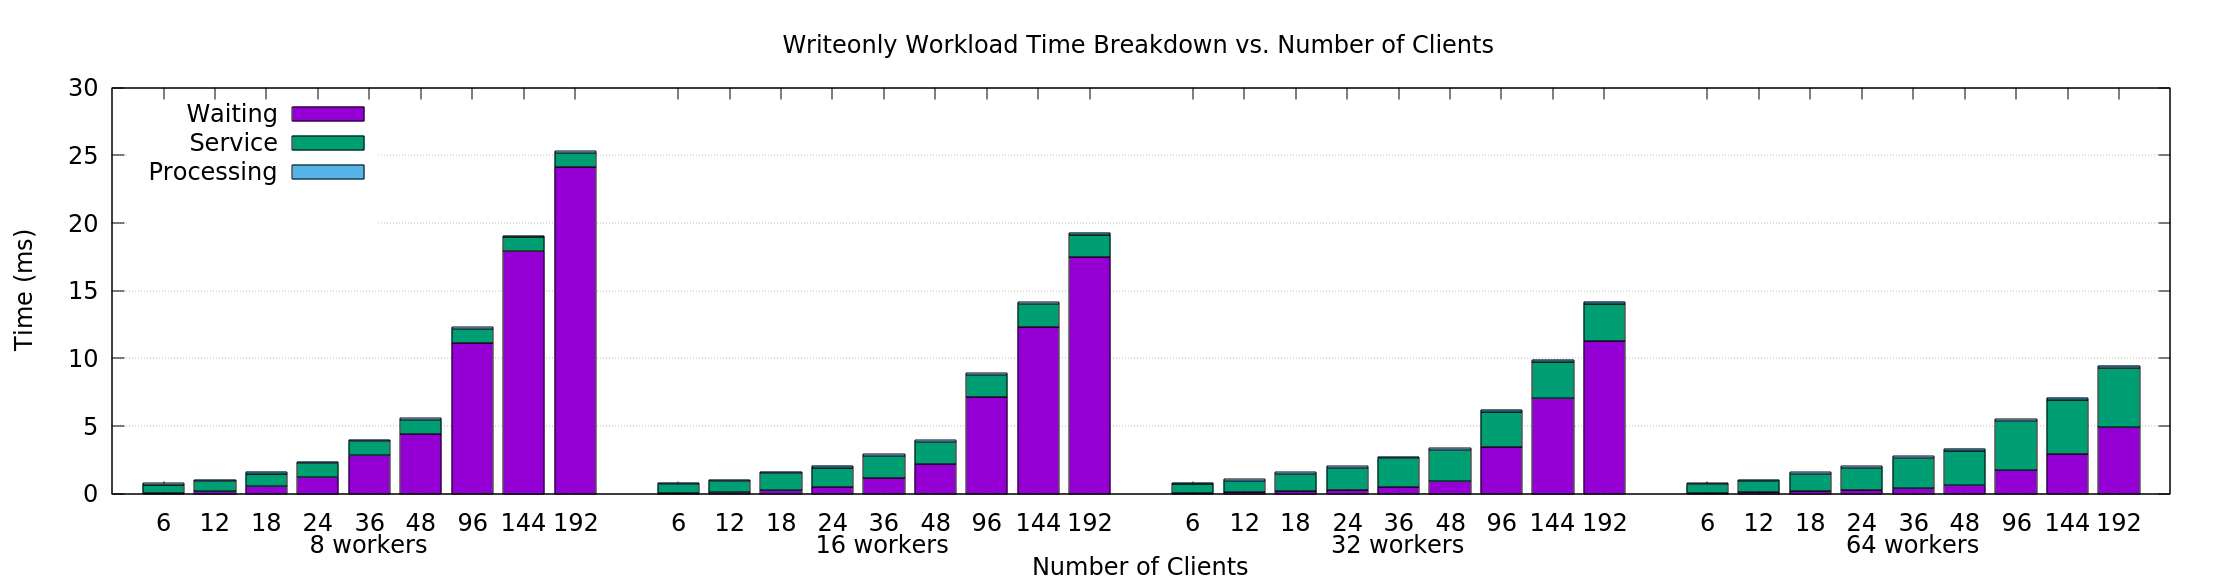
\includegraphics[width=1.0\textwidth]{img/3_1_breakdown_writeonly.png}
\captionsetup{justification=centering}
\caption{\label{fig:3.1writeonly_breakdown}Middleware Time Breakdown for One Middleware Write-only Workload \\(Errors are too small to be seen)}
\end{figure}

For write-only workload, as we increase the number of worker threads, it requires more and more clients to saturate the middleware, because more and more requests can be processed at the same time. Also, we can see that as we add more workers, the performance gain becomes less, because the machine's parallel processing capacity is limited, and adding more threads also introduce more scheduling overhead and resource contention. With the support of Figures~\ref{fig:3.1writeonly_queue} and \ref{fig:3.1writeonly_breakdown}, we can see the worker threads begins to become saturated at 12, 24, 48, 96 clients respectively for 8, 16, 32, 64 worker threads, as both the average queue length and the in-queue waiting time start to scale super-linearly; the middleware becomes fully saturated at 24, 48, 96, 144 clients respectively for 8, 16, 32, 64 threads, as the maximum throughput (7126.27 ops/sec, 9036.63 ops/sec, 10767.83 ops/sec, 12154.73 ops/sec, respectively) has been reached while response time grows linearly. In total, the system reaches the maximum throughput at 144 clients, 64 threads, with 12154.73 ops/sec. The maximum processing capacity of the memcached server is never reached, because now the bottleneck is in the middleware.

%Provide a detailed analysis of the results (e.g., bottleneck analysis, component utilizations, average queue lengths, system saturation). Add any additional figures and experiments that help you illustrate your point and support your claims.

It is worth noting that the bottlenecking component of the middleware can be not only the worker threads, but also the network thread. An important phenomenon we have observed is the response time discrepancy between memtier and middleware measurements. When the middleware is not saturated, we find the difference value is simply equal to the round-trip time between memtier and middleware machines measured by \texttt{ping}, just like the case in Figure~\ref{fig:3.1discrepancy} left, which is trivial to understand. However, further observation, as plotted in Figure~\ref{fig:3.1discrepancy} right, shows that when the middleware is saturated, the discrepancy has a positive correlation with the number of workers, and when the number of worker threads is high, the discrepancy even grows linearly with regard to the number of clients. 

\begin{figure}[!h]
\parbox{.5\linewidth}{
\centering
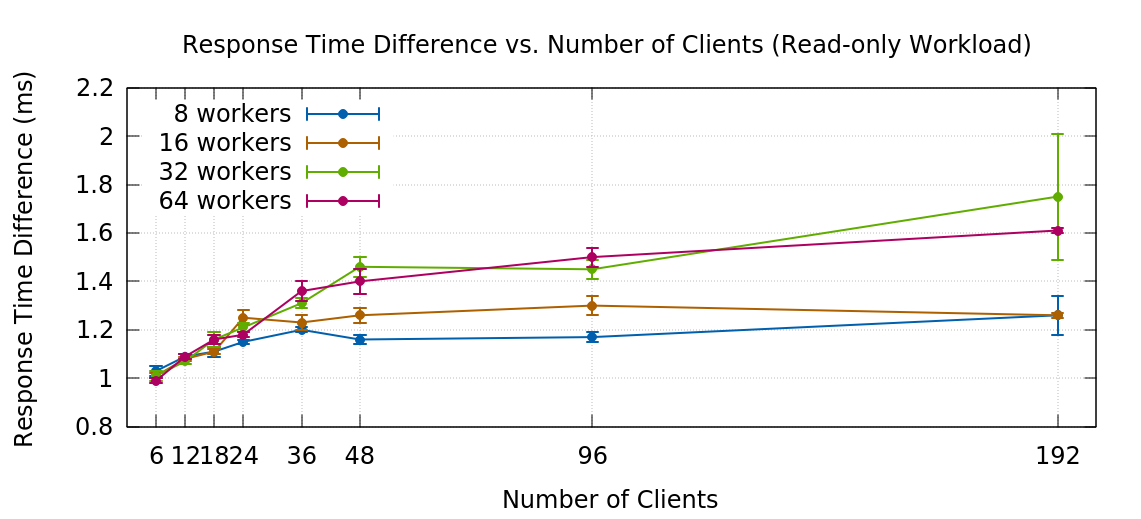
\includegraphics[width=0.5\textwidth]{img/3_1_discrepancy_readonly.png}
}
\parbox{.5\linewidth}{
\centering
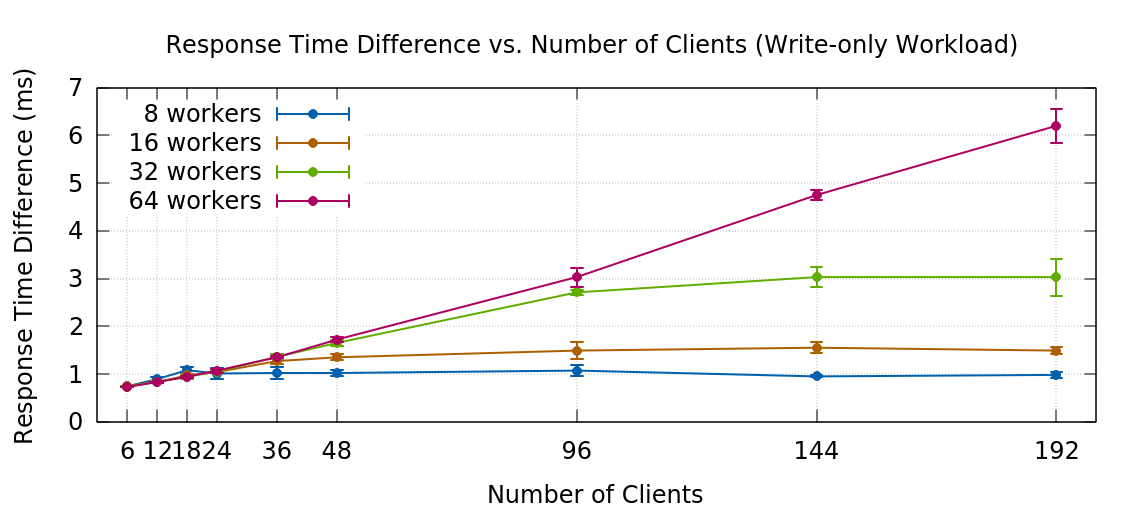
\includegraphics[width=0.5\textwidth]{img/3_1_discrepancy_writeonly.png}
}
\captionsetup{justification=centering}
\caption{\label{fig:3.1discrepancy}Response Time Discrepancy Between Memtier and Middleware Measurements}
\end{figure}

When the middleware is saturated, the discrepancy is not only the RTT. First, adding worker threads increases the throughput, which is also the arrival rate, due to the nature of a closed system. As the arrival rate reaches the processing capacity (service rate) of the network thread, new requests will fill up the operating system network queue, and the network thread cannot immediately handle the \texttt{isReadable} event and read it into the middleware because it may be still parsing the last request. Also, when there are more worker threads, it is more likely to have resource contention since there are only eight cores in the middleware VM, and the network thread could become less responsive due to thread scheduling. So, the requests will have to spend more time waiting in the OS network queue, and this part of waiting time cannot be recorded by the measuring instruments of the middleware, resulting in a larger discrepancy between the measured response times of memtier and the middleware.


\subsection{Two Middlewares}

% Connect three load generator machines (two instances of memtier with CT=1) to two middlewares and use 1 memcached server. Run a read-only and a write-only workload with increasing number of clients (between 2 and 64) and measure response time \emph{both at the client and at the middleware}, and plot the throughput and response time as measured in the middleware.

In this subsection, we double the number of middlewares from the previous subsection and study the performance change. The experiment setup is listed below.
Figure~\ref{fig:3.2readonly} is the response time and throughput measured by the middleware with regard to the number of clients, for read-only workload. Figure~\ref{fig:3.2writeonly} is for write-only workload. The throughput and response time measured by memtier (not shown here) follows the interactive law. Since we have two middlewares now, the pressure on the network thread is relieved, and it does not become the bottleneck, because by simply introducing the network RTT as think time, we confirm that the interactive law also holds for the middleware.

\begin{center}
	\scriptsize{
		\begin{tabular}{|l|c|}
			\hline Number of servers                & 1                        \\ 
			\hline Number of client machines        & 3                        \\ 
			\hline Instances of memtier per machine & 2                        \\ 
			\hline Threads per memtier instance     & 1                        \\
			\hline Virtual clients per thread       & \begin{tabular}{@{}c@{}} For read-only: [1,2,3,4,6,8,16,32]  \\ For write-only: [1,2,4,6,8,16,24,32,36,40] \end{tabular}                 \\ 
			\hline Workload                         & Write-only and Read-only \\
			\hline Multi-Get behavior               & N/A                      \\
			\hline Multi-Get size                   & N/A                      \\
			\hline Number of middlewares            & 2                        \\
			\hline Worker threads per middleware    & [8,16,32,64]                  \\
			\hline Repetitions                      & 3 $\times$ 80 seconds each              \\ 
			\hline 
		\end{tabular}
	} 
\end{center}


\begin{figure}[!h]
\parbox{.5\linewidth}{
\centering
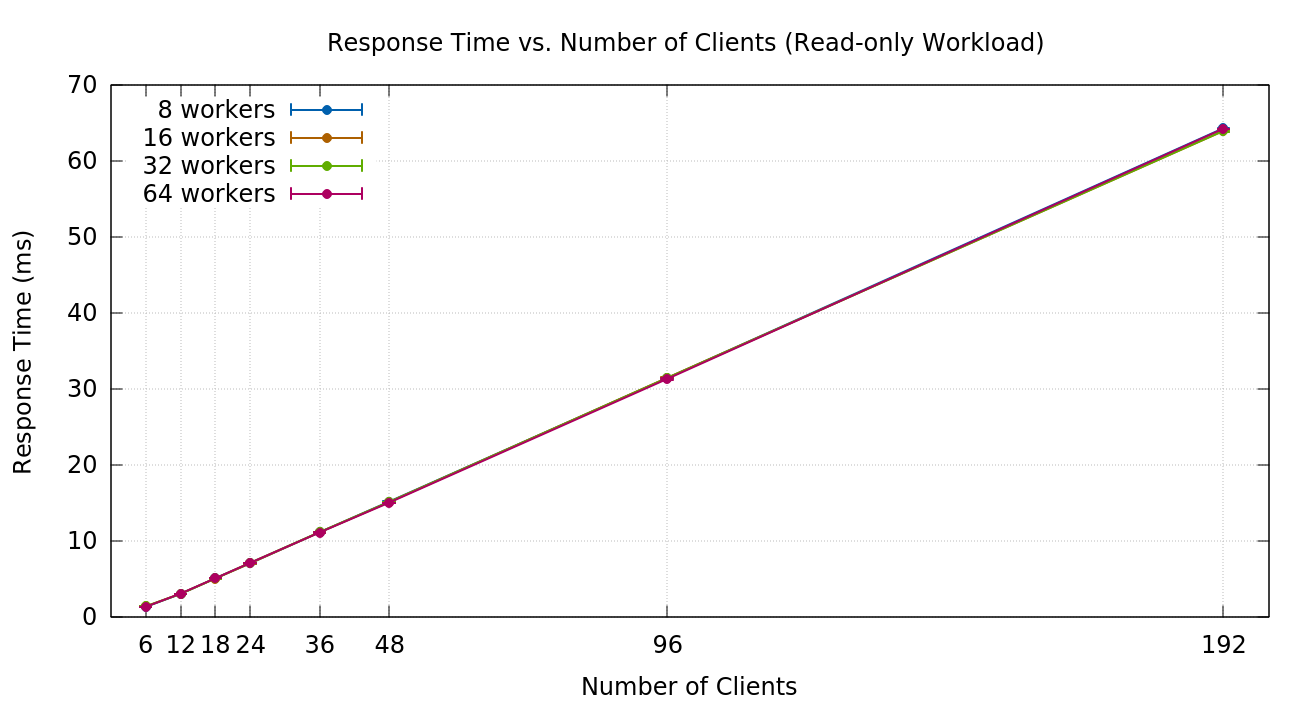
\includegraphics[width=0.5\textwidth]{img/3_2_responsetime_readonly_mw.png}
}
\parbox{.5\linewidth}{
\centering
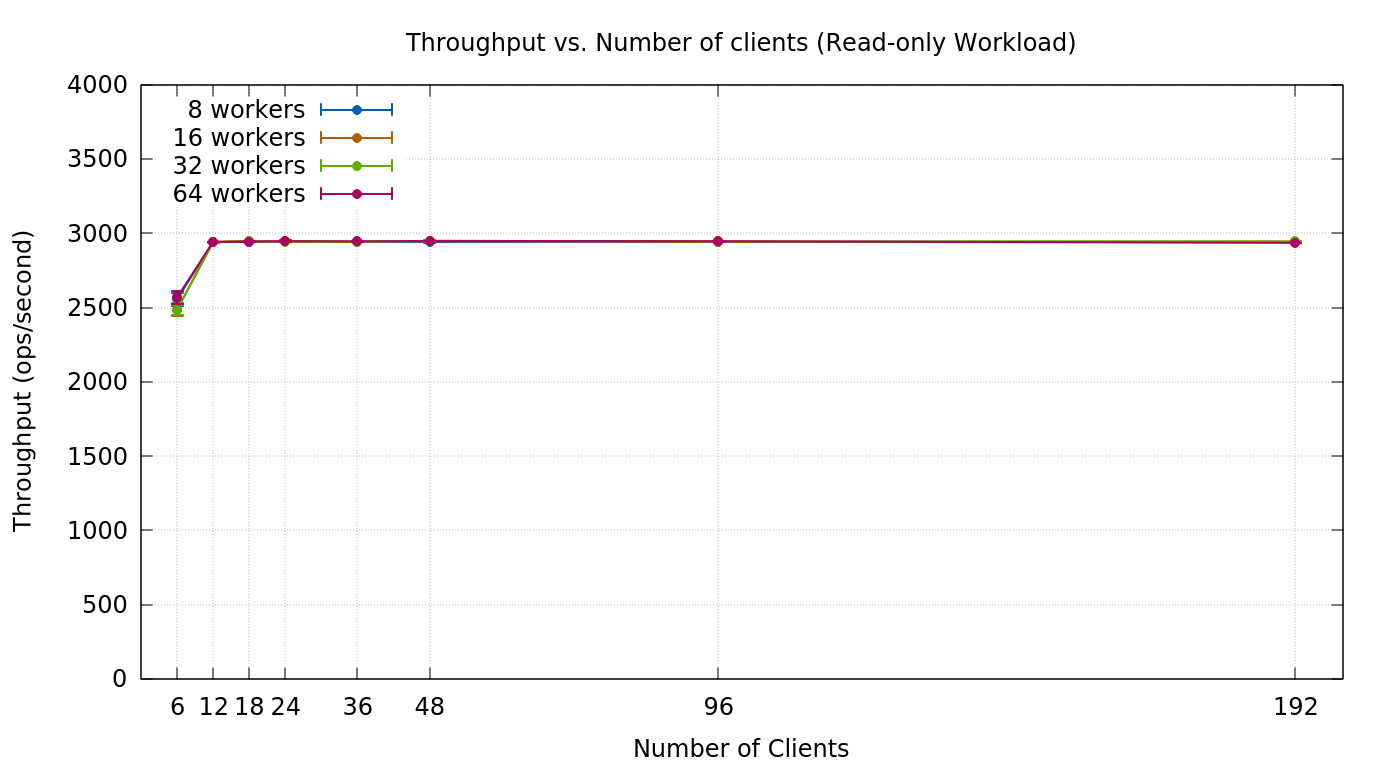
\includegraphics[width=0.5\textwidth]{img/3_2_throughput_readonly_mw.png}
}
\captionsetup{justification=centering}
\caption{\label{fig:3.2readonly}Two Middlewares Read-only Response Time and Throughput Measured on Middleware \\(Error bars are too small to be distinguished)}
% \end{figure}

% \begin{figure}[!h]
\parbox{.5\linewidth}{
\centering
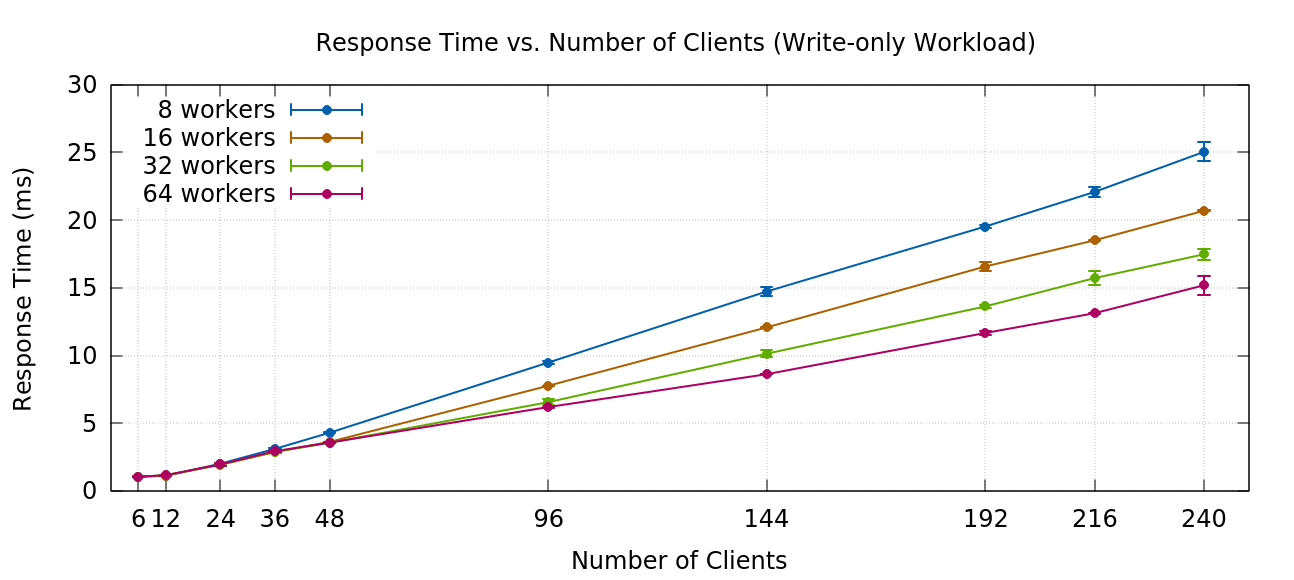
\includegraphics[width=0.5\textwidth]{img/3_2_responsetime_writeonly_mw.png}
}
\parbox{.5\linewidth}{
\centering
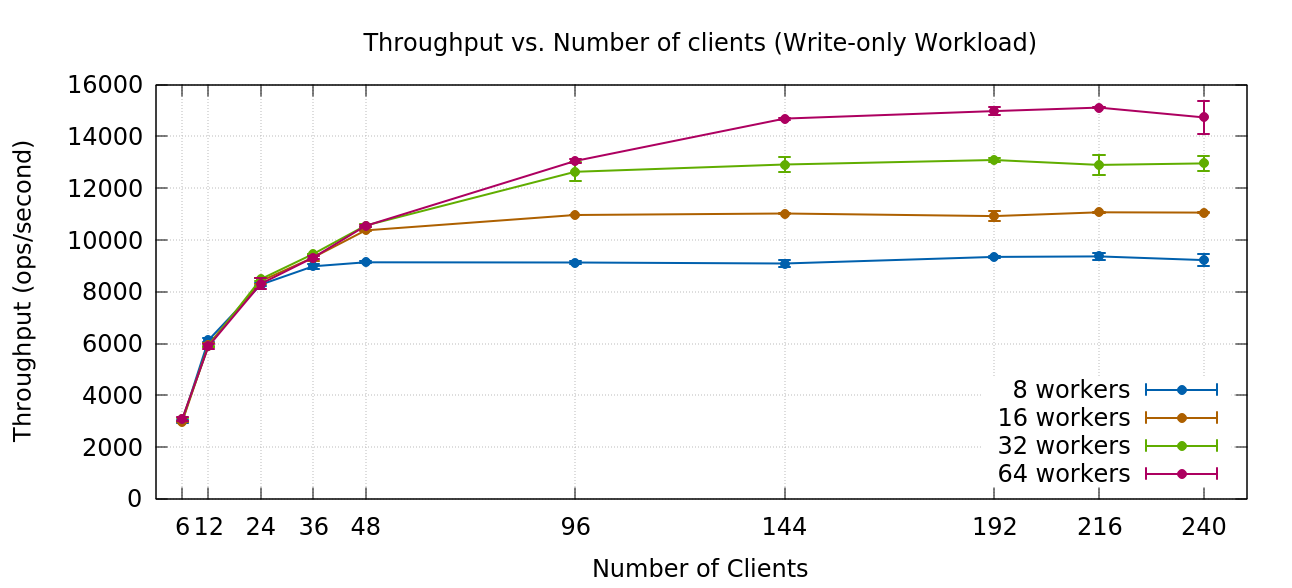
\includegraphics[width=0.5\textwidth]{img/3_2_throughput_writeonly_mw.png}
}
\captionsetup{justification=centering}
\caption{\label{fig:3.2writeonly}Two Middlewares Write-only Response Time and Throughput Measured on Middleware \\(Error bars are too small to be distinguished)}
\end{figure}

\subsubsection{Explanation}

% Provide a detailed analysis of the results (e.g., bottleneck analysis, component utilizations, average queue lengths, system saturation). Add any additional figures and experiments that help you illustrate your point and support your claims.

For read-only workload, the number of worker threads makes no difference, again this is because the throughput is limited by the sending bandwidth of memcached server, and even 8 worker threads are enough to deal with it. For the same reason as explained in Section 3.1.1, the system is saturated at 12 clients, reaching a maximum throughput of 2941.21 ops/sec. The throughput does not increase when adding more clients, while the response time grows linearly.

For write-only workload, the system becomes saturated at 36, 48, 96, 144 clients for 8, 16, 32, 64 worker threads, respectively, because maximum throughput (8981.92 ops/sec, 10368.90 ops/sec, 12630.75 ops/sec, 14688.05 ops/sec, respectively) has been reached and adding clients only results in linear growth of response time. This conclusion is also supported by the middleware time breakdown and average queue lengths as in Figures~\ref{fig:3.2writeonly_queue} and \ref{fig:3.2writeonly_breakdown}, as from these points upwards, the average queue lengths begin to increase dramatically, so do the waiting times in the request queue. The service times are also increased with regard to the number worker threads, indicating the saturation of the memcached server when the load becomes higher. Here we can argue that the bottleneck is not within the middlewares, because the pressure on a single middleware in the previous section has been shared by two middlewares, and with 64 worker threads and 144 clients, the system is able to reach a maximum throughput of about 15000 ops/sec, which is the limit of a memcached server as we have measured in Section 2.1. However, for 8, 16 and 32 threads, the maximum throughput is still limited by insufficient request processing capacity of the middleware.

In the previous subsection, the network thread became saturated when the arrival rate was too high, resulting in large response time discrepancies which is unmeasured by the middleware. However, in this subsection, this does not become a bottleneck because the load is distributed to two middlewares. The fact that the response time discrepancy between memtier and middleware measurements is equal to the \texttt{ping} latencies also supports this conclusion, showing that the waiting time in the OS network queue is about zero.

\begin{figure}[!h]
\centering
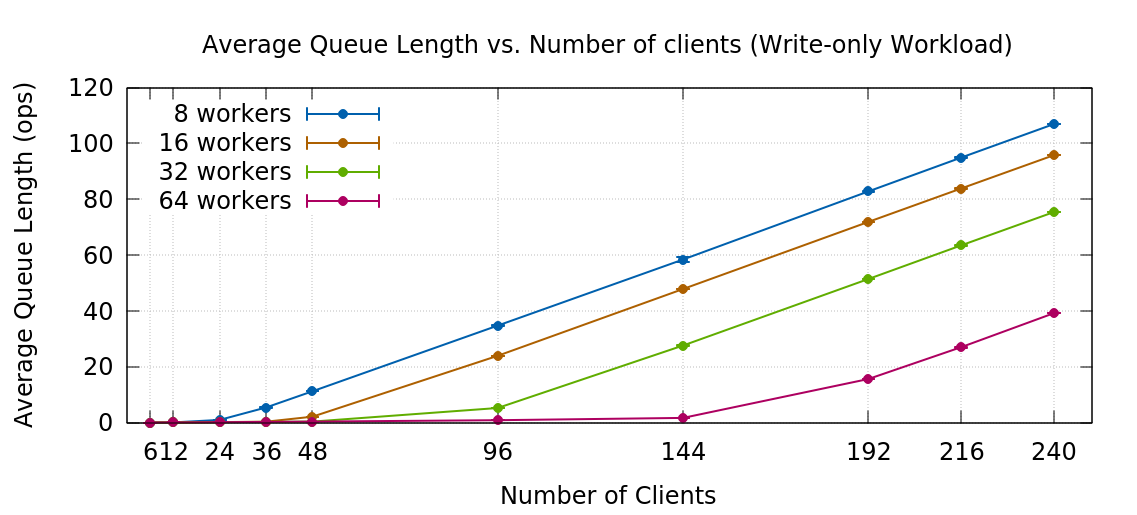
\includegraphics[width=0.7\textwidth]{img/3_2_queuelen_writeonly.png}
\captionsetup{justification=centering}
\caption{\label{fig:3.2writeonly_queue}Average Queue Length for Two Middlewares Write-only Workload \\(Error bars are too small to be distinguished)}
% \end{figure}

% \begin{figure}[!h]
\centering
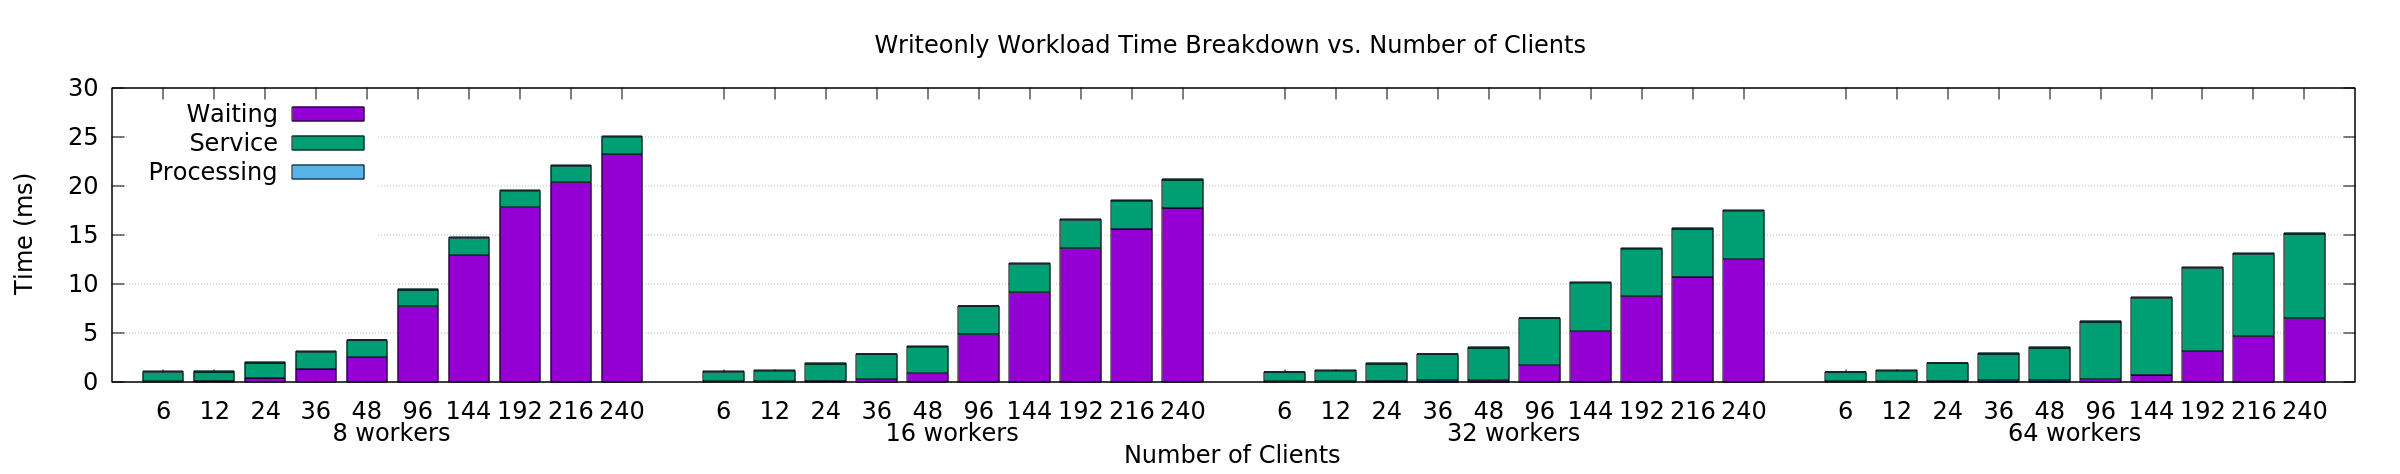
\includegraphics[width=1.0\textwidth]{img/3_2_breakdown_writeonly.png}
\captionsetup{justification=centering}
\caption{\label{fig:3.2writeonly_breakdown}Middleware Time Breakdown for Two Middlewares Write-only Workload \\(Errors are too small to be seen)}
\end{figure}


\subsection{Summary}

% Based on the experiments above, fill out the following table. For both of them use the numbers from a single experiment to fill out all lines. Miss rate represents the percentage of GET requests that return no data. Time in the queue refers to the time spent in the queue between the net-thread and the worker threads.
In the following tables, the maximum throughput experiment is selected so that it is the one that gives the maximum throughput with the least worker threads: 8 threads, 12 clients for read-only workloads in both tables; 64 threads, 144 clients for write-only workloads for one middleware; and 64 threads, 144 clients for write-only workloads for two middlewares.

\begin{center}
	{Maximum throughput for one middleware.}
	\resizebox{0.9\linewidth}{!}{%
	\begin{tabular}{|l|p{2cm}|p{2cm}|p{2cm}|p{2cm}|}
		\hline                                & Throughput & Response time & Average time in queue & Miss rate \\ 
		\hline Reads: Measured on middleware  & 2937.96    &  2.98          & 0.70             &  0         \\ 
		\hline Reads: Measured on clients     & 2903.11    &  4.07         & n/a                   &    0       \\ 
		\hline Writes: Measured on middleware & 12154.73   &  7.09         & 2.95                      & n/a       \\ 
		\hline Writes: Measured on clients    & 12023.66   &  11.84        & n/a                   & n/a       \\ 
		\hline 
	\end{tabular} %
	}
\end{center}

\begin{center}
	{Maximum throughput for two middlewares.}
	\resizebox{0.9\linewidth}{!}{%
	\begin{tabular}{|l|p{2cm}|p{2cm}|p{2cm}|p{2cm}|}
		\hline                                & Throughput (ops/sec) & Response time (ms) & Average time in queue (ms) & Miss rate \\ 
		\hline Reads: Measured on middleware  &  2941.21  &  3.03       & 0.15                  &   0        \\ 
		\hline Reads: Measured on clients     &  2908.47  &  4.07    & n/a                   &   0       \\ 
		\hline Writes: Measured on middleware & 14688.05   &   8.62      & 0.73               & n/a       \\ 
		\hline Writes: Measured on clients    & 14524.03   &   9.81      & n/a                   & n/a       \\ 
		\hline 
	\end{tabular} %
	}
\end{center}

% Based on the data provided in these tables, write at least two paragraphs summarizing your findings about the performance of the middleware in the baseline experiments.

For read-only workload, as we can see from the result, both configurations reach the same maximum throughput with the same number of clients and same response time (with tolerable error). This is because the bottleneck is only at the server side: it cannot send at a higher bandwidth than 100 Mbits/s. It is not even able to saturate a single middleware with only 8 worker threads. A noticable difference is that the average time in queue is much lower in the two middlewares case, and the reason is that the load is distributed to two middlewares, relieving the pressure on a single middleware. In each middleware, the arrival rate is halved, there are less requests waiting in the queue, thus the waiting time is lower.

For write-only workload, two middlewares reach a higher maximum throughput than one. This is because in the one middleware case, the middleware really becomes the bottleneck. Both its network thread and worker threads are compromised: the large response time discrepancy indicates a saturated network thread, which cannot learn the arrival of a request immediately; the large average time in queue indicates saturated worker threads: a request has to wait longer until some worker thread become available to process it. However, with two middlewares, the load is distributed, and the bottleneck again moves back to the memcached server, because the throughput has reached the measured limit of one server in Section 2.1, the response time discrepancy is just the network RTT, and the average waiting time in queue is low.

The experiments in this section also showed us that increasing the number of worker threads, or in its essence, increasing parallelism in request processing, could improve the system's performance. In Section 3.2, we are not able to hit the limit of the memcached server with insufficient number of worker threads, even though we have two middlewares. Before the middleware is saturated, the more worker threads, the more clients we need to saturate the system, and the higher throughput we can get.

Furthermore, the additional plots on average queue length and middleware time breakdowns for work-only workload imply that when the system becomes saturated, its average queue length and waiting time will experience linear or superlinear growth with more clients, which can be used as a indicator of saturation.